\documentclass[a4paper,11pt]{report}
\usepackage[utf8]{inputenc}
%forbibtex
\usepackage[english]{babel}
\usepackage[nottoc]{tocbibind}
%algorithm package
\usepackage{amsmath}
\usepackage{algorithm}
\usepackage[noend]{algpseudocode}
\usepackage{enumerate}
%for code
\usepackage{listings}
\usepackage{color}
\title{REU Project Report}
\author{Nilay Thakor}
\date{July 2016}
%for Graphics
\usepackage{graphicx}
\graphicspath{ {img/} }
%neural network
\usepackage{neuralnetwork}
%url
\usepackage{hyperref}
\hypersetup{
    colorlinks=true,
    linkcolor=blue,
    filecolor=magenta,      
    urlcolor=cyan,
}

\begin{document}

% \maketitle



\begin{titlepage}
\begin{center}
  \bfseries
  \huge UNIVERSITY OF NOTRE DAME
  \vskip.2in
  \textsc{Department of Computer Science}
  \vskip.2in
  \large Interdisciplinary Center for Network Science & Applications (iCeNSA)

  \vskip1in
  \Large REU Project Report
  \vskip1.5in
  \emph{\huge Application of Deep Learning in Class Imabalance}
\end{center}

\vskip1in

\begin{minipage}{.5\textwidth}
  \begin{flushleft}
    \bfseries\large Supervisor:\par \emph{Prof. Nitesh Chawla \\ Prof. Reid Johnson}
  \end{flushleft}
\end{minipage}
\hskip.4\textwidth
\begin{minipage}{.25\textwidth}
  \begin{flushleft}
    \bfseries\large Student:\par \emph{Nilay Thakor}
  \end{flushleft}
\end{minipage}

\vskip1in

\centering
\bfseries
\Large Year \the\year
\end{titlepage}

\chapter*{Introduction}

The issue of class imbalance is observed in data when the class of interest is under represented. This issue has attracted researchers for a long time. The major technique to resolve class imbalance includes resampling of the data.\cite{chawla2009data}. The resampling techniques can be classified as oversampling, undersampling and hybrid techniques. SMOTE\cite{chawla2002smote} is a very famous oversampling algorithm. 

In the recent years various Deep Learning algorithms have achieved breakthrough performances. In this project I have designed some experiments to apply deep learning methods to resolve the issue of class imbalance. 

\chapter*{Experiments}

The experiment are done over various oversampling techniques and integration of deep learning in them. The first set of experiments involves DAEGO\cite{bellinger2015synthetic} method which generates sythetic samples using denoising auto encoders\cite{vincent2010stacked}. 

The other experiments is implementation of DAF\cite{ng2016dual} algorithm which uses stacked denoising encoders to transform the feature space.

In attempt to improve the SMOTE algorithm an experiment SMOTE\_SADE is designed which includes stack de-noising encoders before SMOTE.

\section*{DAEGO}

DAEGO\cite{bellinger2015synthetic} is an oversampling technique to generate synthetic samples using de-noising encoders. The generation of synthetic sample is done using following algorithm.

\begin{algorithm}
\caption{DAEGO}\label{euclid}
\begin{algorithmic}

\begin{enumerate}
    \item {\state $norm\_params \gets \text{Nomalization Parameters}$}
    \item {\state $x\_norm \gets \text{Nomalized Posotive Class using $$norm\_params$$}$}
    \item {\state $dea \gets \text{de-noising encoder network created using hidden layers H and activation $\sigma$}$}
    \item {Train $dea$ using $x\_norm$}
    \item {Transform $x\_init$ using $dea$}
    \item {denormalize $x\_norm$ and $x\_init$ using $norm_params$}
    \item {Return: $x\_init$  }
\end{enumerate}

\end{algorithmic}
\end{algorithm}

The synthetic samples generated by DAEGO has very less variance that compare to SMOTE\cite{chawla2002smote}. Figure ~\ref{fig:smdg} shows that.


\begin{figure}[ht]
\begin{center}
  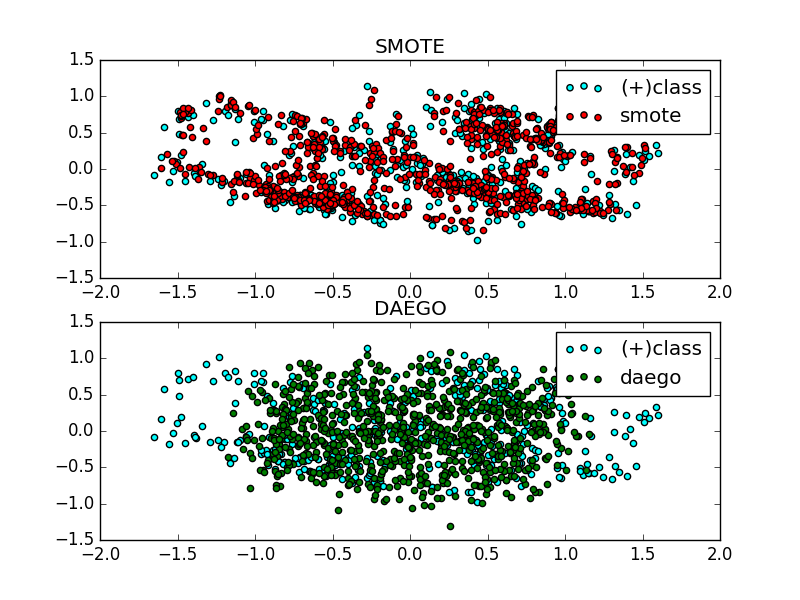
\includegraphics[width=0.5\textwidth]{sm_dg}
\end{center}
    \caption{Comparision between samples generated via SMOTE and DAEGO}
  \label{fig:smdg}
\end{figure}
The experiments shows that AUC score of classifier increases if the when DAEGO samples are generated with higher dimensional hidden layer. Also performance do not vary after more than two hidden layer. 


Additional to DAEGO two experiments were done to increase the dimensionality of data before performing DAEGO using encoder and stacked encoder. 

\subsection*{DAEGO\_ENCODER}


In DAEGO\_ENCODER the I increased the dimensions of data using encoder and than performed DAEGO oversampling. Following diagram explain the process.
\begin{center}
\begin{neuralnetwork}[height=8, layertitleheight=1cm, nodespacing=1cm, layerspacing=2cm]
		\newcommand{\nodetextclear}[2]{}
		\newcommand{\nodetextx}[2]{$x_#2$}
		\newcommand{\nodetexty}[2]{$\hat{x}_#2$}
		\inputlayer[count=4, bias=false, title=Input\\layer, text=\nodetextx]
		\hiddenlayer[count=7, bias=false, title=Encoding\\layer, text=\nodetextclear] \linklayers
		\hiddenlayer[count=7, bias=false, title=DAEGO, text=\nodetextclear] \linklayers
		\hiddenlayer[count=7, bias=false, title=Decoding\\layer, text=\nodetextclear] \linklayers
		\outputlayer[count=4, title=Output\\layer, text=\nodetexty] \linklayers
	\end{neuralnetwork}
\end{center}
\subsection*{DAEGO\_SDAE}

In DAEGO\_SDAE the we increase the dimensions of data using stacked encoders and than performed DAEGO oversampling. Following diagram explain the process.


\begin{neuralnetwork}[height=8, layertitleheight=1cm, nodespacing=1cm, layerspacing=2cm]
		\newcommand{\nodetextclear}[2]{}
		\newcommand{\nodetextx}[2]{$x_#2$}
		\newcommand{\nodetexty}[2]{$\hat{x}_#2$}
		\inputlayer[count=4, bias=false, title=Input\\layer, text=\nodetextx]
		\hiddenlayer[count=5, bias=false, title=Encoding\\layer 1, text=\nodetextclear] \linklayers
		\hiddenlayer[count=7, bias=false, title=Encoding\\layer 2, text=\nodetextclear] \linklayers
		\hiddenlayer[count=7, bias=false, title=DAEGO, text=\nodetextclear] \linklayers
		\hiddenlayer[count=7, bias=false, title=Decoding\\layer 1, text=\nodetextclear] \linklayers
		\hiddenlayer[count=5, bias=false, title=Decoding\\layer 2, text=\nodetextclear] \linklayers
		\outputlayer[count=4, title=Output\\layer, text=\nodetexty] \linklayers
	\end{neuralnetwork}
	
\subsection*{SDAEGO}

In this experiment we use deep stacked denoising encoders to geneate synthetic samples. It follows the same procedure as DAEGO but uses stacked encoders for synthetic data.

\section*{DAF}

DAF\cite{ng2016dual} is a resampling technique which uses stacked de-noising encoders to resample the data into reduced feature space. Figure ~\ref{fig:daf} shows the procedure. It transform the dataset using stacked encoders and \textit{sigmoid} and \textit{tanh} activation respectively. By stacking both the output we get final resampled dataset.  

\begin{figure}[ht]
\begin{center}
  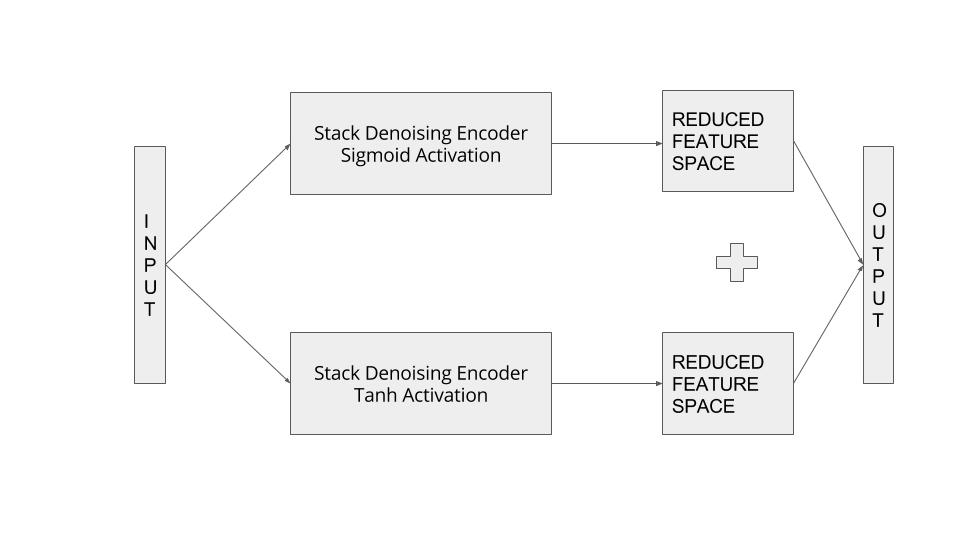
\includegraphics[width=\textwidth]{daf}
\end{center}
    \caption{DAF}
  \label{fig:daf}
\end{figure}



\begin{algorithm}
\caption{DAF}\label{euclid}
\begin{algorithmic}

\begin{enumerate}
    \item {Create a stacked encoder network using hidden layers H}
    \item {Scale the dataset between the range of 0 to 1 }
    \item {Train the dataset using sdae network using 
    sigmoid activation and tanh activation}
    \item {merge both the output}
\end{enumerate}

\end{algorithmic}
\end{algorithm}

\section*{SMOTE\_SDAE}

This experiment transform the dataset into higher dimesional space using staced encoder than perform the SMOTE oversampling. Following diagram explains the procedure.


\begin{neuralnetwork}[height=8, layertitleheight=1cm, nodespacing=1cm, layerspacing=2cm]
		\newcommand{\nodetextclear}[2]{}
		\newcommand{\nodetextx}[2]{$x_#2$}
		\newcommand{\nodetexty}[2]{$\hat{x}_#2$}
		\inputlayer[count=4, bias=false, title=Input\\layer, text=\nodetextx]
		\hiddenlayer[count=5, bias=false, title=Encoding\\layer 1, text=\nodetextclear] \linklayers
		\hiddenlayer[count=7, bias=false, title=Encoding\\layer 2, text=\nodetextclear] \linklayers
		\hiddenlayer[count=7, bias=false, title=SMOTE, text=\nodetextclear] \linklayers
		\hiddenlayer[count=7, bias=false, title=Decoding\\layer 1, text=\nodetextclear] \linklayers
		\hiddenlayer[count=5, bias=false, title=Decoding\\layer 2, text=\nodetextclear] \linklayers
		\outputlayer[count=4, title=Output\\layer, text=\nodetexty] \linklayers
	\end{neuralnetwork}

\chapter*{Results}

All the experiments were tested on four different dataset. Table ~\ref{tab:dataset} has information about all datasets. The imbalance ratio is defined as Negative Class Samples to  Positive Class Sample  ratio. 


\begin{table}[h]
\centering
\caption{Datasets}
\label{tab:dataset}
\begin{tabular}{|c|c|c|c|}
\hline
\textbf{Dataset} & \textbf{Features} & \textbf{Sample} & \textbf{Imbalance Ratio} \\ \hline
Segment          & 19                & 2310            & 6                        \\ \hline
KDDCUP           & 76                & 145751          & 111.46                   \\ \hline
boundary         & 175               & 3505            & 27.495                   \\ \hline
page-block       & 10                & 1578            & 8.788                    \\ \hline
\end{tabular}
\end{table}

The classifier used are Decision Tree and Multilayer Perceptron. The ratio of training vs testing data is 70:30. 

Table ~\ref{tab:res1} Compares results of classifiers without any resampling and 100\% oversampling of SMOTE, DAEGO and SDAEGO

\begin{table}[h]
\centering
\caption{Results}
\label{tab:res1}
\resizebox{\textwidth}{!}{%
\begin{tabular}{|c|c|c|c|c|c|c|c|c|c|}
\hline
Dataset    & CLF & NONE         &              & SMOTE        &              & DAEGO        &              & SDAEGO        &              \\ \hline
           &     & PC           & AUC          & PC           & AUC          & PC           & AUC          & PC            & AUC          \\ \hline
Segment    & DT  & 0.9739130435 & 0.9976958525 & 0.9655172414 & 0.9969278034 & 0.9655172414 & 0.9969278034 & 0.6967213115  & 0.8689950422 \\ \hline
           & MLP & 1            & 0.9955357143 & 0.9824561404 & 0.9984639017 & 1            & 0.9910714286 & 1             & 0.98598      \\ \hline
KDDCUP     & DT  & 0.612371134  & 0.871144928  & 0.6336842105 & 0.8763168041 & 0.6812652068 & 0.8503856284 & 0.1818181818  & 0.8533867244 \\ \hline
           & MLP & 0.6012658228 & 0.8560590689 & 0.5593869732 & 0.8644232694 & 0.7878787879 & 0.76071953   & 0.97          & 0.7193940625 \\ \hline
boundary   & DT  & 0.008888     & 0.53         & 0.125        & 0.54529      & 0.078947     & 0.5209       & 0.05769230769 & 0.5165474061 \\ \hline
           & MLP & 0.375        & 0.5958672    & 0.086        & 0.51498      & 0.1          & 0.51632      & 0.2           & 0.5220632081 \\ \hline
page-block & DT  & 0.8206521739 & 0.8892668178 & 0.8062827225 & 0.8959664674 & 0.8636363636 & 0.8946952518 & 0.3586387435  & 0.7866762867 \\ \hline
           & MLP & 0.7571428571 & 0.9048649763 & 0.8333333333 & 0.9004672576 & 0.8529411765 & 0.8758675187 & 0.9150943396  & 0.7538308253 \\ \hline
\end{tabular}%
}
\end{table}




Table ~\ref{tab:res2} compares 100\% oversampling of two feature transformation method applied before DAEGO.
% Please add the following required packages to your document preamble:
% \usepackage{graphicx}
\begin{table}[h]
\centering
\caption{Results}
\label{tab:res2}
\resizebox{\textwidth}{!}{%
\begin{tabular}{|c|c|c|c|c|c|c|c|c|c|}
\hline
Dataset    & CLF & NONE         &              & SMOTE        &              & DAEGO\_SDAE   &              & DAEGO\_ENCODER &        \\ \hline
           &     & PC           & AUC          & PC           & AUC          & PC            & AUC          & PC             & AUC    \\ \hline
Segment    & DT  & 0.9739130435 & 0.9976958525 & 0.9655172414 & 0.9969278034 & 0             & 0.5          & 0.1467889908   & 0.5    \\ \hline
           & MLP & 1            & 0.9955357143 & 0.9824561404 & 0.9984639017 & 0.1467889908  & 0.5          & 0.1773162939   & 0.6    \\ \hline
page-block & DT  & 0.8206521739 & 0.8892668178 & 0.8062827225 & 0.8959664674 & 0.4285714286  & 0.5066996496 & 0.0841924      & 0.3944 \\ \hline
           & MLP & 0.7571428571 & 0.9048649763 & 0.8333333333 & 0.9004672576 & 0.09870276368 & 0.4688380403 & 0.1046511      & 0.5    \\ \hline
\end{tabular}%
}
\end{table}

Table ~\ref{tab:res3} comapres results of resampling method DAF and SMOTE\_SDAE.
% Please add the following required packages to your document preamble:
% \usepackage{graphicx}
\begin{table}[h]
\centering
\caption{Results}
\label{tab:res3}
\resizebox{\textwidth}{!}{%
\begin{tabular}{|c|c|c|c|c|c|c|c|c|c|}
\hline
Dataset    & CLF & NONE         &              & SMOTE        &              & DAEGO\_SDAE   &              & DAEGO\_ENCODER &        \\ \hline
           &     & PC           & AUC          & PC           & AUC          & PC            & AUC          & PC             & AUC    \\ \hline
Segment    & DT  & 0.9739130435 & 0.9976958525 & 0.9655172414 & 0.9969278034 & 0             & 0.5          & 0.1467889908   & 0.5    \\ \hline
           & MLP & 1            & 0.9955357143 & 0.9824561404 & 0.9984639017 & 0.1467889908  & 0.5          & 0.1773162939   & 0.6    \\ \hline
page-block & DT  & 0.8206521739 & 0.8892668178 & 0.8062827225 & 0.8959664674 & 0.4285714286  & 0.5066996496 & 0.0841924      & 0.3944 \\ \hline
           & MLP & 0.7571428571 & 0.9048649763 & 0.8333333333 & 0.9004672576 & 0.09870276368 & 0.4688380403 & 0.1046511      & 0.5    \\ \hline
\end{tabular}%
}
\end{table}


The detailed results and code can be found at \url{https://github.com/nthakor/imbalance_algorithms}


\section*{Future work}

Above experiments are an effort to integrate the deep learning approaches to resolve class imbalance via over-sampling. Following are some areas need to be explored to improve the results geerated by these experiments.

\begin{itemize}
    \item {In some of the datasets issue of class overlapping is observed. The re-sampling method using deep learning can be developed to resolve the issue.}
    \item{The most experiments performed are related includes oversampling. The effectiveness of deep learning approaches can be explored in other methods like under-sampling. }
    \item{The above experiments apply deep learning approaches in the process of oversampling. Unsupervised deep learning approaches can be applied after oversampling.}
\end{itemize}



%Sets the bibliography style to UNSRT and imports the 
%bibliography file "samples.bib".
\bibliographystyle{unsrt}
\bibliography{sample}
\end{document}
